\documentclass[paper=a4, fontsize=11pt]{scrartcl} % A4 paper and 11pt font size
\usepackage{./../usfassignment}
\settitle{Assignment 4}
\setauthor{Wanzhang Sheng}
\setcourse{CS675: Automata Theory}

\begin{document}

\maketitle % Print the title

% -----------------------------------------------------------------------------
% PROBLEM 1
% -----------------------------------------------------------------------------
\section{}

\begin{fancyquotes}
  For each of the following languages, first give an NFA, and then
  find an equivalent regular expression using the method discussed in
  class. Show the resulting machine after each state has been
  removed. Finally, simplify the resulting regular expression as much
  as possible.
\end{fancyquotes}

\begin{figure}[hp]
  \centering
  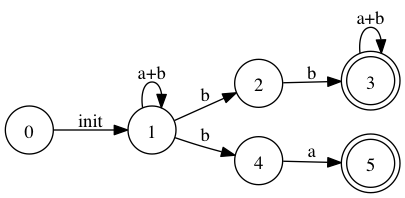
\includegraphics[width=.4\textwidth]{1-1.gv.png}
  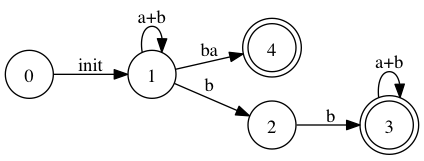
\includegraphics[width=.4\textwidth]{1-1.gv.2.png}
  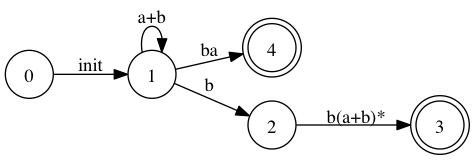
\includegraphics[width=.4\textwidth]{1-1.gv.3.png}
  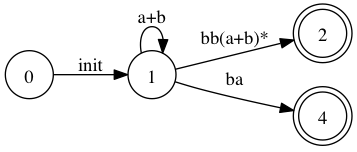
\includegraphics[width=.4\textwidth]{1-1.gv.4.png}
  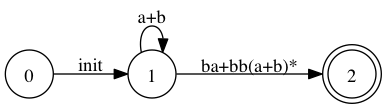
\includegraphics[width=.4\textwidth]{1-1.gv.5.png}
  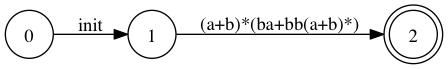
\includegraphics[width=.4\textwidth]{1-1.gv.6.png}
  \caption{(8 points) $L$ = All strings over ${a,b}$ that contain the substring $bb$ or end in $ba$.}
\end{figure}
The simplest expression is $(a+b)^*(ba+bb(a+b)^*)$.

\begin{figure}[hp]
  \centering
  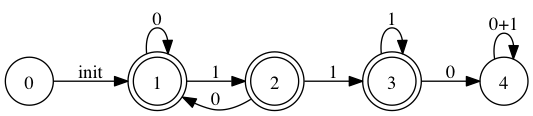
\includegraphics[width=.4\textwidth]{1-2.gv.png}
  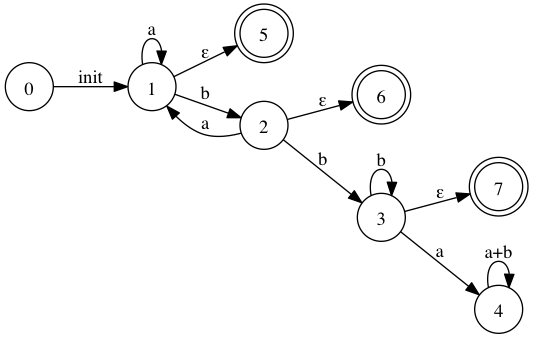
\includegraphics[width=.4\textwidth]{1-2.gv.2.png}
  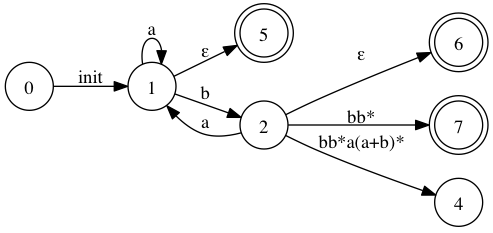
\includegraphics[width=.4\textwidth]{1-2.gv.3.png}
  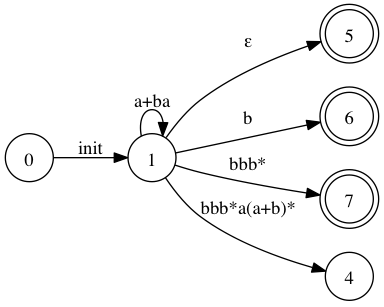
\includegraphics[width=.4\textwidth]{1-2.gv.4.png}
  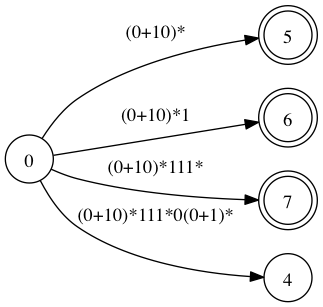
\includegraphics[width=.4\textwidth]{1-2.gv.5.png}
  \caption{(8 points) $L$ = All strings over ${0,1}$ that do not contain the substring $bba$}
\end{figure}
The simplest expression is $(a+ba)^*(\epsilon + bb^*)$.

\begin{figure}[hp]
  \centering
  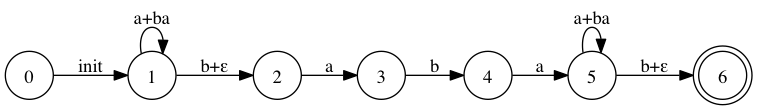
\includegraphics[width=.4\textwidth]{1-3.gv.png}
  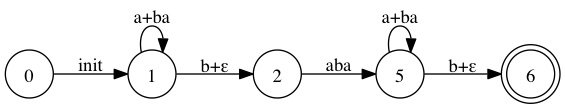
\includegraphics[width=.4\textwidth]{1-3.gv.2.png}
  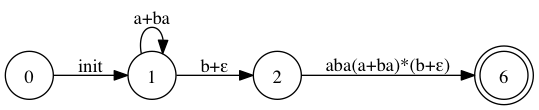
\includegraphics[width=.4\textwidth]{1-3.gv.3.png}
  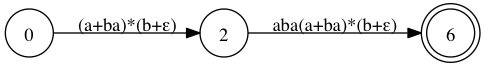
\includegraphics[width=.4\textwidth]{1-3.gv.4.png}
  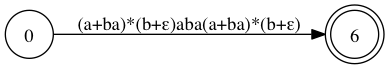
\includegraphics[width=.4\textwidth]{1-3.gv.5.png}
  \caption{(8 points) $L$ = All strings over ${a,b}$ that contain $aba$ but not $bb$}
\end{figure}
The simplest expression is $(a+ba)^*(b+\epsilon)aba(a+ba)^*(b+\epsilon)$.


% -----------------------------------------------------------------------------
% PROBLEM 2
% -----------------------------------------------------------------------------
\section{}

\begin{fancyquotes}
  Let $L_R$ be some regular language, and let $L_{NR}$ be some
  non-regular language. Prove or disprove each of the following
  statements (use a counter-example to disprove):
\end{fancyquotes}

\begin{enumerate}
\item
  \begin{fancyquotes}
    (3 points) If $L \subseteq L_R$, then $L$ must be regular.
  \end{fancyquotes}

  True.

  Since $L \subseteq L_R \in L_{REG}$,
  so if $L\subseteq L_R$, $L$ must be regular.

\item
  \begin{fancyquotes}
    (3 points) If $L \subseteq L_{NR}$, then $L$ cannot be regular.
  \end{fancyquotes}

  True.

  $L \subseteq L_{NR} \in \overline{L_{REG}} = L_{NREG} =
  \{L: \text{L is a non-regular language.}\}$

  So if $L \subseteq L_{NR}$, then $L$ cannot be regular.

\item
  \begin{fancyquotes}
    (3 points) If $L \subseteq L_{NR} \cap L_R$, then $L$ must be regular.
  \end{fancyquotes}

  False.

  Given $L_{NR}=\{s: 0^n1^n2^n, \text{over}\;\{0,1,2\}\}$,
  $L_{R}=R[{(0+1)}^*]$. So $L_{NR}\cap L_R = \{s: 0^n1^n,
  \text{over}\;\{0,1,2\}\}$, which is a non regular language.

\item
  \begin{fancyquotes}
    (3 points) If $L \subseteq L_{NR} \cap L_R$, then $L$ cannot be regular.
  \end{fancyquotes}

  False.

  Given $L_{NR}=\{s: 0^*1^n2^n, \text{over}\;\{0,1,2\}\}$,
  $L_{R}=R[{(0+1)}^*]$. So $L_{NR}\cap L_R = R[0^*1^*]$, which is a
  regular language.

\item
  \begin{fancyquotes}
    (3 points) If $L = \overline{L_{NR}}$ (that is, $L$ is the complement of $L_{NR}$),
    then $L$ cannot be regular.
  \end{fancyquotes}

  True.

  Assume that $L = \overline{L_{NR}}$ is a regular language.
  Since regular languages are closed under complementation, then
  $\overline{L} = \overline{\overline{L_{NR}}} = L_{NR} \in L_{NREG}$.

  Contradicted. So $L = \overline{L_{NR}}$ is not a regular language.

\item
  \begin{fancyquotes}
    (3 points) If $L_1$ is regular, then the language $L_2 = \{xy :
    x\in L_1, y \not\in L_1\}$ is regular.
  \end{fancyquotes}

  True.

  Let $L_1 = R[r_1]$ and $\overline{L_1} = R[r_2]$ since regular
  languages are closed under complementation.
  Then $L_2 = R[r_1r_2]$ which is regular.
\end{enumerate}


% -----------------------------------------------------------------------------
% PROBLEM 3
% -----------------------------------------------------------------------------
\section{}

\begin{fancyquotes}
  For each of the following languages, prove that the language is
  regular, or prove that the language is not regular. Recall that you
  prove a langauge is regular by creating either a DFA, NFA, or
  regular expression for that language. Careful, some of these are
  tricky\dots
\end{fancyquotes}

\begin{enumerate}
\item
  \begin{fancyquotes}
    (4 points) $L = \{a^n(a+b)^*b^n, n\geq 2\}$
  \end{fancyquotes}

  It is non-regular.

  Assume that it's a regular language.

  Let $k$ be the constant of the pumping lemma.

  Given a string $w = a^kb^k \in L$, which $k>n$.

  If we break $w = xyz$ such that $|xy|<k, |y|>0$, then
  $x = a^i, y = a^j, z = a^{k-i-j}b^k$.

  Consider a new string $w_2 = xy^2z = a^{k+j}b^k$,
  as long as $j>0$ it cannot be in $L$.

  Hence, $L$ is not regular by pumping lemma.

\item
  \begin{fancyquotes}
    (4 points) $L = \{ww^R : w\in\{a,b\}^*\}$
  \end{fancyquotes}

  It is non-regular.

  Assume that it's a regular language.

  Let $n$ be the constant of the pumping lemma.

  Given a string $s = a^nbba^n \in L$.

  If we break $s = xyz$ such that $|xy|<n, |y|>0$, then
  $x = a^i, y = a^j, z = a^{n-i-j}bba^n$.

  Consider a new string $s_2 = xy^2z = a^{n+j}bba^n$,
  as long as $j>0$ it cannot be in $L$.

  Hence, $L$ is not regular by pumping lemma.

\item
  \begin{fancyquotes}
    (4 points) $L = \{wxw^R : w\in\{a,b\}^*, x\in\{a,b\}^*\}$
  \end{fancyquotes}


  It is regular.

  In fact $L = \{wxw^R : w\in\{a,b\}^*, x\in\{a,b\}^*\} = \{x :
  x\in\{a,b\}^*\} = R[(a+b)^*]$.

\item
  \begin{fancyquotes}
    (4 points) $L = \{a^{n}b^l : n/l is an integer\}$
  \end{fancyquotes}

  It is non-regular.

  Assume that it's a regular language.

  Let $n$ be the constant of the pumping lemma.

  Given a string $s = a^{kn}b^n \in L$, which $k\in N^+$.

  If we break $s = xyz$ such that $|xy|<n, |y|>0$, then
  $x = a^i, y = a^j, z = a^{kn-i-j}b^n$.

  Consider a new string $s_2 = xy^2z = a^{kn+j}b^n$,
  as long as $0<j<n$, $0<\frac{j}{n}<1$ cannot be integer, so $s_2$ cannot be in $L$.

  Hence, $L$ is not regular by pumping lemma.

\item
  \begin{fancyquotes}
    (4 points) $L = \{a^{n}b^l : n\geq 100, l\leq 100\}$
  \end{fancyquotes}

  It is regular.

  $L = R[a^*\underbrace{aa\ldots a}_{100 a}
  (b+bb+\ldots+\underbrace{bb\ldots b}_{100 b})]$

\end{enumerate}


% -----------------------------------------------------------------------------
% PROBLEM 4
% -----------------------------------------------------------------------------
\section{}

\begin{fancyquotes}
  (4 points) Question 2.4.2 from the text Let $D = \{0,1\}$, and let
  $T = D\times D\times D$. A correct addition of two numbers in binary
  notation can be considered a string in $T^*$, if we think of the
  symbols in $T$ as vertical columns. For example,

  \begin{center}
    \begin{tabular}[hp]{rrrrr}
      &0 &1 &0 &1\\
      + &0 &1 &1 &0\\
      \hline
      &1 &0 &1 &1\\
    \end{tabular}
  \end{center}

  would be pictured by the following four symbols:

  \[
  \begin{pmatrix}0\\0\\1\end{pmatrix}
  \begin{pmatrix}1\\1\\0\end{pmatrix}
  \begin{pmatrix}0\\1\\1\end{pmatrix}
  \begin{pmatrix}1\\0\\1\end{pmatrix}
  \]

  Show that strings in $T^*$ that represent correct addtion is a
  regular language. (Hint: You probably want to use a DFA or NFA for
  this (but of course a regular expression is fine, too). Your string
  is read by the automata from left-to-right (and not right-to-left),
  so you will need to keep track of the carry bit in a speculative
  way. As always, come to me with questions.)
\end{fancyquotes}

Let $\{X_{-1},X_0,X_1,X_2\}$ be a partition of $T$, and
$X_i = \{(a_1,a_2,a_3)^T: (a_1,a_2,a_3)^T\in T, a_1+a_2-a_3=i\}$.
So that:
\[X_{-1} = \{(0,0,1)^T\}\]
\[X_0 = \{(0,0,0)^T, (0,1,1)^T, (1,0,1)^T\}\]
\[X_1 = \{(0,1,0)^T, (1,0,0)^T, (1,1,1)^T\}\]
\[X_2 = \{(1,1,0)^T\}\]

Let $M = (K,\Sigma,\Delta,s,F)$ be a NFA, and $K = \{-1,0\}$, $\Sigma
= T $, $\Delta = \{((q_1,t),q_2): q_1,q_2\in K, t\in X_i, 2\times
q_1+i=q_2 \} $, $s = s$, $F = \{0\}$.
The graph will look like this:

\begin{figure}[hp]
  \centering
  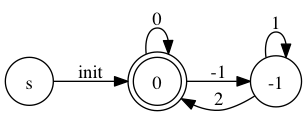
\includegraphics[width=.4\textwidth]{1-4.gv.png}
  \caption{addition correct NFA}
\end{figure}

Or in regular expression: $(R_{0}+((R_{-1})R_{1}^*R_{2})^*)^*$, which
$L[R_i] = X_i$.

Even further, we can have NFA for addition check of arbitrary $k$ hex.
Just extend the symbol sets and change the $2$ in $\Delta$ to the hex $k$.


% -----------------------------------------------------------------------------
% PROBLEM 5
% -----------------------------------------------------------------------------
\section{}

\begin{fancyquotes}
  (4 points) Show that the following language is not regular: $L = \{w
  : w \in (a + b)^* \text{and the number of a's in w is composite}\}$.
\end{fancyquotes}

Assume that it's a regular language.
Then since regular languages are closed under complementation,
we have $L_2 = \overline{L}$ is a regular language.

Let $n$ be the constant of the pumping lemma.

Given a string $s = a^{m} \in L_2$, which $m>n$.

If we break $s = xyz$ such that $|xy|<n, |y|>0$, then
$x = a^i, y = a^j, z = a^{m-i-j}$.

Consider a new string $s_2 = xy^{m+1}z = a^{m+mj} = a^{m(1+j)}$,
as long as $j>0$, $1+j>1$, the number of $a$ in $s_2$ must be
composite, so $s_2$ cannot be in $L_2$.

Hence, $L_2$ is not regular by pumping lemma.

Contradiction. So $L$ is not regular.


\end{document}
